% F1R3Games Agentic Players — Test harness design, version 1
% Build: xelatex agentic-players-design.tex (twice). Fonts in ./fonts, logos in ./logos
% (copied from github.com/F1R3FLY-io/f1r3fly-brand-portal).
\documentclass[11pt,a4paper]{article}
\newcommand{\docheader}{Agentic players · Harness design · v1}
\newcommand{\docdate}{9 October 2026}
% F1R3FLY.io house preamble for printable technical documents.
% Follows the F1R3Games design documents (brand kit v1.2, 12 June 2026):
% white interior, Yellow and Sky as rules and fills only, never as text.
% Expects \docheader and \docdate to be defined before \input.
\usepackage[a4paper,top=30mm,bottom=26mm,left=22mm,right=22mm,headsep=10mm,footskip=12mm]{geometry}
\usepackage{fontspec}
\usepackage{xcolor}
\usepackage{graphicx}
\usepackage{tikz}
\usetikzlibrary{arrows.meta,positioning,calc,fit,backgrounds,decorations.pathreplacing}
\usepackage{titlesec}
\usepackage{fancyhdr}
\usepackage{enumitem}
\usepackage{booktabs}
\usepackage{tabularx}
\usepackage{array}
\usepackage{listings}
\usepackage[most]{tcolorbox}
\usepackage{amsmath,amssymb,amsthm}
\usepackage[hidelinks]{hyperref}
\usepackage{etoolbox}
\usepackage{microtype}

\definecolor{brandyellow}{HTML}{F3D630}
\definecolor{brandsky}{HTML}{3FA9F5}
\definecolor{brandskydark}{HTML}{00528C}
\definecolor{brandblack}{HTML}{000000}
\definecolor{muted}{HTML}{3F3F3F}
\definecolor{footgray}{HTML}{595959}
\definecolor{codebg}{HTML}{F2F2F2}
\definecolor{rulegray}{HTML}{C5C5C5}

\setmainfont{SourceSans3}[
  Path=./fonts/, Extension=.ttf,
  UprightFont=*-400, BoldFont=*-700, ItalicFont=*-400,
  ItalicFeatures={FakeSlant=0.18}, BoldItalicFont=*-700, BoldItalicFeatures={FakeSlant=0.18}]
\newfontfamily\spartanbold{LeagueSpartan-Bold}[Path=./fonts/, Extension=.ttf]
\newfontfamily\spartansemi{LeagueSpartan-SemiBold}[Path=./fonts/, Extension=.ttf]
\newfontfamily\spartanreg{LeagueSpartan-Regular}[Path=./fonts/, Extension=.ttf]
\newfontfamily\spartanlight{LeagueSpartan-Light}[Path=./fonts/, Extension=.ttf]
\newfontfamily\sourcelight{SourceSans3-300}[Path=./fonts/, Extension=.ttf]
\setmonofont{DejaVu Sans Mono}[Scale=0.84]
\renewcommand{\sffamily}{\spartanreg}

\newcommand{\caps}[1]{{\addfontfeatures{LetterSpace=12}\MakeUppercase{#1}}}
\newcommand{\gradrule}[1][\linewidth]{%
  \noindent\begin{tikzpicture}\shade[left color=brandyellow,right color=brandsky]
  (0,0) rectangle (#1,0.6pt);\end{tikzpicture}}

\hypersetup{colorlinks=true,linkcolor=brandskydark,urlcolor=brandskydark,citecolor=brandskydark,pdfauthor={F1R3FLY.io}}

\titleformat{\section}{\spartanbold\fontsize{13}{16}\selectfont}
  {\caps{\thesection}\hspace{1em}}{0pt}{\caps}[\vspace{3pt}\gradrule]
\titleformat{\subsection}{\spartansemi\fontsize{10.5}{13}\selectfont}{\thesubsection\hspace{0.8em}}{0pt}{}
\titleformat{\subsubsection}[runin]{\bfseries}{}{0pt}{}[.]
\titlespacing*{\section}{0pt}{20pt}{12pt}
\titlespacing*{\subsection}{0pt}{14pt}{6pt}
\setcounter{secnumdepth}{2}
\setcounter{tocdepth}{2}

\setlength{\parindent}{0pt}
\setlength{\parskip}{6pt}
\linespread{1.08}
\emergencystretch=3em

\pagestyle{fancy}
\fancyhf{}
\renewcommand{\headrulewidth}{0pt}
\fancyhead[L]{\raisebox{-2pt}{
\includegraphics[height=7.5mm]{logos/f1r3fly-io-horizontal-logo-white-background.pdf}}}
\fancyhead[R]{\spartanreg\fontsize{8}{10}\selectfont\color{footgray}\caps{\docheader}}
\fancyfoot[L]{\spartanbold\fontsize{7.5}{9}\selectfont\color{footgray}\thepage}
\fancyfoot[R]{\spartanbold\fontsize{7.5}{9}\selectfont\color{footgray}\textcopyright{} F1R3FLY INDUSTRIES, 2026. All Rights Reserved \textbar{} \docdate}

\lstdefinelanguage{rholang}{
  morekeywords={new,in,for,contract,match,if,else,bundle,Nil,true,false,not,and,or},
  sensitive=true, morecomment=[l]{//}, morestring=[b]"}
\lstdefinelanguage{toml}{morecomment=[l]{\#}, morestring=[b]", sensitive=true}
\lstset{basicstyle=\ttfamily\small,backgroundcolor=\color{codebg},frame=leftline,
  rulecolor=\color{brandsky},framerule=1.2pt,framesep=6pt,xleftmargin=8pt,
  breaklines=true,columns=fullflexible,keepspaces=true,showstringspaces=false,
  keywordstyle=\bfseries,commentstyle=\color{muted},aboveskip=8pt,belowskip=8pt}

\newcommand{\code}[1]{\texttt{#1}}
\newcommand{\MUST}{{\fontsize{0.82em}{1em}\selectfont MUST}}
\newcommand{\MUSTNOT}{{\fontsize{0.82em}{1em}\selectfont MUST NOT}}
\newcommand{\SHOULD}{{\fontsize{0.82em}{1em}\selectfont SHOULD}}
\newcommand{\MAY}{{\fontsize{0.82em}{1em}\selectfont MAY}}

\newtcolorbox{decision}[2]{enhanced,breakable,colback=white,colframe=white,
  boxrule=0pt,left=10pt,right=4pt,top=4pt,bottom=4pt,
  borderline west={2.2pt}{0pt}{brandsky},
  fontupper=\small,
  title={\spartanbold\fontsize{8.5}{10}\selectfont\color{brandblack}\caps{Decision #1}\quad
         \spartansemi\normalsize\fontsize{10.5}{12}\selectfont #2},
  coltitle=brandblack,colbacktitle=white,attach title to upper,after title={\par\smallskip}}

\newtcolorbox{finding}[2]{enhanced,breakable,colback=codebg,colframe=codebg,
  boxrule=0pt,left=8pt,right=6pt,top=5pt,bottom=5pt,arc=2pt,
  title={\spartanbold\fontsize{8.5}{10}\selectfont\caps{Finding #1}\quad\spartansemi\fontsize{10.5}{12}\selectfont #2},
  coltitle=brandblack,colbacktitle=codebg,attach title to upper,after title={\par\smallskip},fontupper=\small}

\newtcolorbox{claimbox}[1]{enhanced,breakable,colback=white,colframe=white,
  boxrule=0pt,left=10pt,right=4pt,top=4pt,bottom=4pt,
  borderline west={2.2pt}{0pt}{brandyellow},
  title={\spartanbold\fontsize{8.5}{10}\selectfont\color{brandblack}\caps{#1}},
  coltitle=brandblack,colbacktitle=white,attach title to upper,after title={\par\smallskip}}

\theoremstyle{definition}
\newtheorem{definition}{Definition}
\newtheorem{proposition}[definition]{Proposition}
\newtheorem{remark}[definition]{Remark}
\newtheorem{hypothesis}{Hypothesis}

% Cover. #1 kicker, #2 title, #3 subtitle, #4 details block.
\newcommand{\ffiocover}[4]{%
\begin{titlepage}
\newgeometry{margin=0pt}
\pagecolor{brandblack}\color{white}
\begin{tikzpicture}[remember picture,overlay]
  \node[anchor=north] at ($(current page.north)+(0,-38mm)$)
    {
\includegraphics[width=70mm]{logos/f1r3fly-io-vertical-logo-color-on-dark.pdf}};
  \node[anchor=north west,text width=150mm,text=white] at ($(current page.north west)+(30mm,-148mm)$) {%
    {\spartanbold\fontsize{9}{11}\selectfont\color{brandyellow}\caps{#1}}\par\vspace{8mm}
    {\spartanlight\fontsize{34}{40}\selectfont #2}\par\vspace{5mm}
    {\sourcelight\fontsize{15}{20}\selectfont #3}\par\vspace{9mm}
    \begin{tikzpicture}\shade[left color=brandyellow,right color=brandsky] (0,0) rectangle (150mm,0.6pt);\end{tikzpicture}\par\vspace{7mm}
    {\fontsize{10.5}{15}\selectfont #4}};
  \node[anchor=south east] at ($(current page.south east)+(-22mm,14mm)$)
    {\spartanbold\fontsize{7.5}{9}\selectfont\color[HTML]{C5C5C5}\textcopyright{} F1R3FLY INDUSTRIES, 2026. All Rights Reserved \textbar{} \docdate};
\end{tikzpicture}
\restoregeometry
\end{titlepage}
\nopagecolor\color{black}}

\newcommand{\summarybox}[1]{%
\begin{center}\begin{minipage}{0.9\linewidth}
{\spartanbold\fontsize{8.5}{10}\selectfont\caps{Summary}}\par\smallskip #1
\end{minipage}\end{center}}

\hypersetup{pdftitle={F1R3Games Agentic Players: Test Harness Design}}

\begin{document}

\ffiocover{F1R3Games · Harness design}
  {Agentic Players}
  {A test harness for social and compositional intelligence on a F1R3FLY shard}
  {Version 1 \quad·\quad 9 October 2026\par
   Conforms to F1R3Games \code{f1r3ink-impl@d2381c6} (Portal, F1R3Pix, F1R3Beat, F1R3Ink)\par
   and F1R3Node-Rust \code{feature/cost-accounted-rho@55431d1}\par
   Companion: \emph{Many Hands}, research note, 9 October 2026}

\summarybox{%
This document specifies a harness that lets agents play the F1R3Games as first-class players, so
that the games can test the theses of the companion research note: that intelligence is social,
that it is compositional, and that a reified collective can interact with its own components.
Agents of four kinds take part: rule-following f1r3lang agents, locally executed open-source
models, frontier models, and aggregators that reify a collective by aggregating its members'
behaviour, each aggregation a commitment to one view of the state. Each agent holds its own key,
joins games through the same Portal protocol as a person, and is bound by the same wallet policy.

Three mechanisms make the population an experimental variable. A \emph{mixer} funds each
subpopulation from a lane of its own, so the shares of activity are set by the inflows into lanes
and not by how fast agents can act or how many identities they hold. A \emph{disclosure switch},
held by the host of each instance, decides what players are told about who is an agent; the
attestations behind it are sealed on chain until the switch or the close of the experiment releases
them. An \emph{Observatory} captures every record and computes the research note's observables,
including the composition defect against an arm whose social channels are severed.

Version~1 runs against the Portal and node as they stand, funding lanes through sponsorships and
wallet allowances. Version~2 moves lanes into the cost-accounted calculus when the node's funding
slots are complete. Section~\ref{sec:decisions} lists the decisions; five were settled by the
author of the games on 9 October and the rest are recommended for review.}

\vspace{2mm}
\begingroup\footnotesize\linespread{0.92}\selectfont\setlength{\parskip}{0pt}\setcounter{tocdepth}{1}\tableofcontents\endgroup
\newpage

% =====================================================================
\section{Decisions}\label{sec:decisions}

\begin{center}\small
\begin{tabularx}{\linewidth}{@{}l>{\raggedright\arraybackslash}p{36mm}X@{}}
\toprule
 & question & decision or recommendation\\
\midrule
D1 & \textbf{Settled.} Which agents & Both locally executed open-source models and frontier
  models. \emph{Recommended:} also rule-following f1r3lang agents (K0), the only population with no
  imported discourse, and aggregators (A).\\
D2 & \textbf{Settled.} How a collective is reified & By aggregation of its members' behaviour,
  each aggregation a commitment to one view of the state; not by rho's quotation. The result is
  seated as an ordinary player. \emph{Recommended:} five aggregator kinds in version~1, each logging
  its commitments (\S\ref{sec:aggregators}).\\
D3 & \textbf{Settled.} Rate limiting & Token-gated coordination: subpopulations are funded from
  lanes, and a mixer sets the inflows. \emph{Recommended:} lanes through sponsorships and
  allowances in version~1; native lanes in version~2 (\S\ref{sec:mixer}).\\
D4 & \textbf{Settled.} Disclosure & A switch held by the host. \emph{Recommended:} four levels;
  sealed attestations with on-chain commitments; full reveal at close by default
  (\S\ref{sec:disclosure}).\\
D5 & \textbf{Settled.} Observables & Whole games and collections of games: the seesaw of complexity
  and compression, and the STER analogues. \emph{Recommended:} computed after the fact, never shown
  to players during an arm (\S\ref{sec:observatory}).\\
D6 & Where agents plug in & A Rust service, \code{f1r3games-agents}, in the Portal workspace,
  reusing \code{f1r3games-core}, \code{-wallet} and \code{-games}; it calls \code{f1r3games-service}
  exactly as the shell does.\\
D7 & Agent keys & One key per agent per instance by default, so an anonymous agent cannot be traced
  across games; persistent keys for longitudinal arms.\\
D8 & Agent signing & Every agent signs as \code{Origin::Game} under an allowance, like a person
  playing in a game frame; payments only through a capped, logged path.\\
D9 & Where models run & Off chain, in the harness, by default. On-chain inference through
  \code{rho:ollama} is a research option for version~2, after replay is verified.\\
D10 & K0 agents & Policies written in rholang and evaluated as exploratory deploys in version~1;
  persistent on-chain processes on funding slots in version~2.\\
D11 & Severed arms & A new instance setting, \code{channels = "severed"}, honoured by every game's
  \code{say} and by \code{payments.send}.\\
D12 & Selection pressure & Engagement is recorded with the engager's lane, and breeders weight it
  by lane.\\
D13 & Thinking costs & Model spend is metered and capped per lane in the harness, and reported
  beside shard cost; it is not a shard token in version~1.\\
D14 & Players' messages to agents & Treated as data. An agent's only actions are the moves of its
  game, so a message cannot make it do anything else.\\
D15 & People in research instances & Consent at join; a platform notice that agents may be
  present; a debrief when disclosure was withheld.\\
\bottomrule
\end{tabularx}
\end{center}

% =====================================================================
\section{Purpose, sources and conformance}\label{sec:purpose}

\subsection{What the harness is for}

The companion note argues that intelligence is bootstrapped from components that carry nothing
recognisable as intelligence and improved by composition, and that a collective can be reified and
seated among its components. The F1R3Games are an instrument for that argument at everyday scale.
Each player has almost no individual power, so structure on the board is evidence of coordination,
and every act is recorded on a F1R3FLY shard. The harness makes the population of players a
variable under control: which kinds of agents play, in what mix, at what rates, with what
disclosure, and with which collectives seated among them.

\subsection{Sources reviewed}

\begin{itemize}[itemsep=1pt]
\item F1R3Games, branch \code{f1r3ink-impl@d2381c6} (8 October 2026), which contains the Portal
  (\code{Portal/f1r3games-portal}: crates \code{core}, \code{wallet}, \code{node}, \code{service},
  \code{games}, \code{cli}, \code{rholint}; the React shell in \code{web}; \code{templates/env.rho}
  and the game environments), the designs of the Portal, F1R3Pix, F1R3Beat and F1R3Ink, and
  \code{docs/IMPLEMENTATION.md}.
\item F1R3Node-Rust, branch \code{feature/cost-accounted-rho@55431d1} (9 October 2026): the HTTP
  API, the deploy envelope, the cost-accounting implementation guide
  in \code{docs/casper/theory/} and the wallet-funded process guide.
\item Embers and F1R3Sky: the AI-agent and agent-team domains of Embers, and the wallets of both.
\item ign1t10n, branch \code{f1r3games}: the supervised processes and ports.
\item F1R3FLY-io/publications at \code{2cb0f6e}: the cost-accounting papers, the virtual-token
  note, mortal computation, the rho-life series, the chess society and the quorum note.
\end{itemize}

\subsection{Order of authority}

Where sources disagree, F1R3Node-Rust prevails, then F1R3Sky and Embers, then the Portal, then
the game designs. The harness changes no node behaviour. It adds two environment domains and three
instance settings to the Portal (\S\ref{sec:env}), and otherwise uses the Portal as a person's
shell does.

\subsection{Conventions}

\MUST, \SHOULD{} and \MAY{} are used as in RFC~2119. Requirements are numbered R1, R2, \dots{} and
collected where they arise.

% =====================================================================
\section{What the review found}\label{sec:findings}

\begin{finding}{F1}{A headless client already exists}
The CLI runs headless with \code{F1R3GAMES\_KEY} (IMPLEMENTATION.md, F6): one key in memory, pinned
to the live environment. Its \code{call} and \code{read} commands reach every game method, and
F1R3Beat's breeder already runs this way under ign1t10n. It signs as \code{Origin::Portal} with no
allowance, so play moves prompt unless \code{-y} is passed. The harness keeps the path and changes
the origin.
\end{finding}

\begin{finding}{F2}{Writes are authenticated by the deploy, not by a session}
There is no login server. A write is a prepared deploy, checked by the wallet's policy, signed with
secp256k1 and sent. The service's token only binds the prepared bytes, the deployer and an expiry.
Every environment method derives its caller from \code{rho:deploy:data}. An agent with a key is
therefore exactly as authenticated as a person with a key, and no more.
\end{finding}

\begin{finding}{F3}{Allowances are the budget mechanism a person already has}
A launch grants an \code{Allowance\{game, instance, templates, budget, spent, expires\_at\}} so
that a game's play templates sign without a prompt; the default is 5,000,000 phlo for four hours.
Fund-moving templates (\code{MOVES\_FUNDS}) are refused unless the origin is the Portal.
\end{finding}

\begin{finding}{F4}{Reads poll and lag finality}
Reads are exploratory deploys against the observer's last finalised block. Game clients poll every
3\,s; there is no streaming in the Portal or the clients, though the node offers \code{/ws/events}.
An agent sees what a person sees, at the same lag.
\end{finding}

\begin{finding}{F5}{Rate limits are few and local}
The only rate limits in the Portal are the F1R3Ink relay's \code{per\_hour} (default 30) and HTTP
429s; F1R3Ink also paces each stripe by \code{minInterval} on block time. The node has none beyond
its block-proposal heartbeat and the observer's capacity. Nothing yet bounds a population's share of
activity.
\end{finding}

\begin{finding}{F6}{The node's cost accounting is one token with many lanes}
On \code{feature/cost-accounted-rho}, per-COMM gating is implemented in Rholang and RSpace, and the
Casper bindings are design contracts to be completed on \code{feature/casper-cost-accounting-completion}.
The production refinement does not introduce a second token or ledger: native REV flows from wallets
into process purses and funding slots, each an authority lane, and settlement burns what is
consumed. Owners can fund a process purse and restrict which operations draw on it. Offered-funded
deploys (\code{POST /api/deploy/offered}) exist, with qualification still pending. Priced conversion
between assets is specified but not implemented.
\end{finding}

\begin{finding}{F7}{There is no notion of an agent player}
Nothing in the Portal or the game environments distinguishes a person from an agent. Embers has AI
agents and agent teams (stored Rholang that calls \code{rho:ai:gpt4} and similar), and the node has
\code{rho:ollama:chat}, \code{generate} and \code{models}, disabled by default. The old F1R3SideChat
prototype described an AI co-author persona; the current SideChat environment has none.
\end{finding}

\begin{finding}{F8}{Sponsorships are almost lanes}
\code{sponsors.create} escrows funds with terms \code{\{stipend, maxPerAddress, expiresAt\}}, and
\code{sponsors.claim} pays a stipend to any participant of an instance. A lane needs one more term:
who is eligible.
\end{finding}

% =====================================================================
\section{Requirements}\label{sec:req}

\begin{enumerate}[label=\textbf{R\arabic*},leftmargin=2.6em,itemsep=2pt]
\item An agent \MUST{} act only through the Portal's prepare, policy, sign and send path, or, for
  version~2 on-chain agents, through deploys the game environments accept from anyone.
\item An agent \MUST{} hold its own key and \MUSTNOT{} share a key with another agent or a person.
\item An agent's actions \MUST{} be limited to its game's move templates and, where the arm permits,
  \code{payments.send} within a cap.
\item Every subpopulation \MUST{} draw shard funds from its own lane, and the mixer \MUST{} be able to
  set each lane's inflow per epoch.
\item The harness \MUST{} cap and log model spend per lane.
\item The host's disclosure level \MUST{} govern what any client can learn about who is an agent
  before the instance closes.
\item Every model call \MUST{} be logged with the model's identity, version, parameters and the
  hashes of its input and output.
\item An experiment \MUST{} be reproducible from its configuration, its seeds and its logs, up to the
  nondeterminism of external models, which \MUST{} be recorded.
\item Observables \MUSTNOT{} be visible to players or agents during an arm.
\item People in research instances \MUST{} consent at join and \MUST{} be told agents may be present.
\end{enumerate}

% =====================================================================
\section{Architecture}\label{sec:arch}

\begin{figure}[ht]
\centering
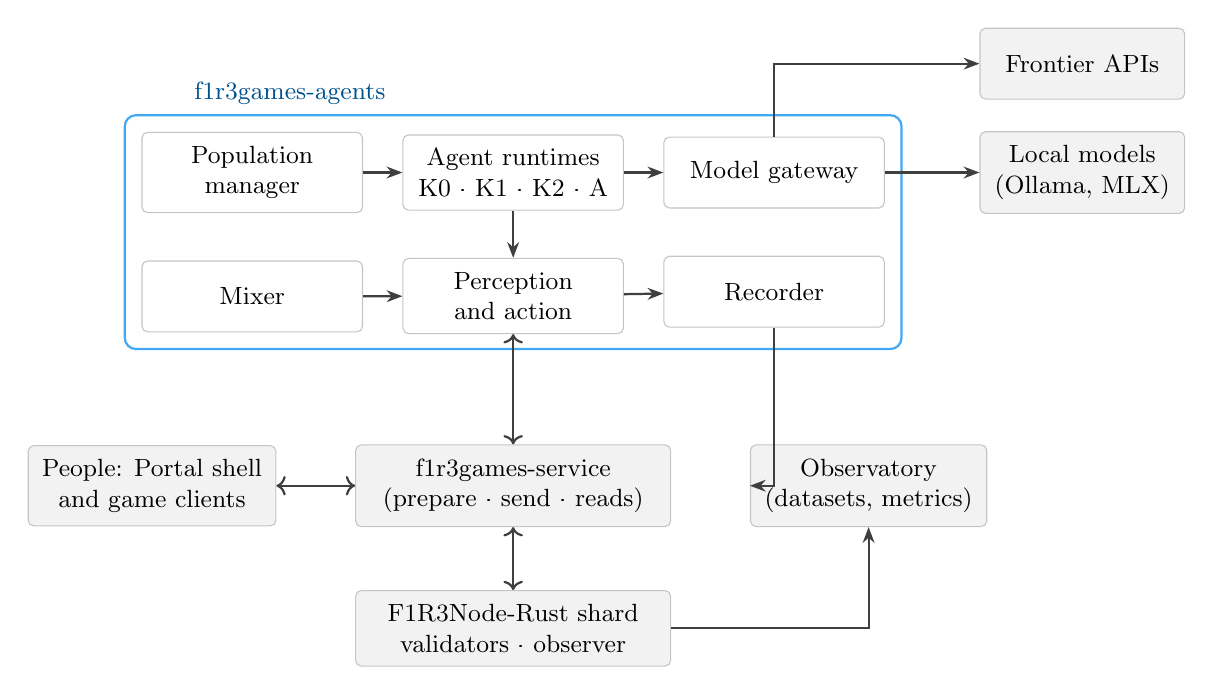
\begin{tikzpicture}[font=\small,
  box/.style={draw=rulegray,fill=white,rounded corners=2pt,align=center,inner sep=5pt,minimum height=9mm},
  hbox/.style={box,fill=codebg},
  arr/.style={-{Stealth[length=2mm]},muted,thick}]
  % harness
  \node[box,minimum width=28mm] (pop) {Population\\manager};
  \node[box,right=5mm of pop,minimum width=28mm] (rt) {Agent runtimes\\K0 · K1 · K2 · A};
  \node[box,right=5mm of rt,minimum width=28mm] (gw) {Model gateway};
  \node[box,below=6mm of pop,minimum width=28mm] (mix) {Mixer};
  \node[box,below=6mm of rt,minimum width=28mm] (act) {Perception\\and action};
  \node[box,below=6mm of gw,minimum width=28mm] (rec) {Recorder};
  \begin{scope}[on background layer]
    \node[draw=brandsky,thick,rounded corners=4pt,fit=(pop)(gw)(mix)(rec),inner sep=6pt,
      label={[font=\spartansemi\small,text=brandskydark]above left:{f1r3games-agents}}] (h) {};
  \end{scope}
  % models
  \node[hbox,right=12mm of gw,minimum width=26mm] (local) {Local models\\(Ollama, MLX)};
  \node[hbox,above=4mm of local,minimum width=26mm] (front) {Frontier APIs};
  % portal + node
  \node[hbox,below=14mm of act,minimum width=40mm] (svc) {f1r3games-service\\(prepare · send · reads)};
  \node[hbox,below=8mm of svc,minimum width=40mm] (node) {F1R3Node-Rust shard\\validators · observer};
  \node[hbox,right=10mm of svc,minimum width=30mm] (obs) {Observatory\\(datasets, metrics)};
  \node[hbox,left=10mm of svc,minimum width=30mm] (shell) {People: Portal shell\\and game clients};
  \draw[arr] (gw) -- (local); \draw[arr] (gw) |- (front);
  \draw[arr] (rt) -- (gw); \draw[arr] (pop) -- (rt); \draw[arr] (rt) -- (act);
  \draw[arr] (mix) -- (act); \draw[arr] (act) -- (rec);
  \draw[arr,<->] (act) -- (svc); \draw[arr,<->] (svc) -- (node);
  \draw[arr,<->] (shell) -- (svc);
  \draw[arr] (rec) |- (obs); \draw[arr] (node) -| (obs);
\end{tikzpicture}
\caption{The harness beside the Portal. Agents reach the shard through \code{f1r3games-service},
as people do through the shell. The mixer funds lanes; the recorder and the shard feed the
Observatory.}
\label{fig:arch}
\end{figure}

The harness is one Rust service, \code{f1r3games-agents}, added to the Portal workspace and run
beside \code{f1r3games-service}. It has six parts.

\begin{description}[leftmargin=1.2em,itemsep=3pt,font=\normalfont\spartansemi]
\item[Population manager.] Reads an experiment configuration (\S\ref{sec:experiments}), creates
  agents and their keys, joins them to instances, starts and stops arms.
\item[Agent runtimes.] One runtime per agent kind, each running the agent loop of
  \S\ref{sec:loop}.
\item[Model gateway.] One interface to every model, local or frontier, with pinning, logging and
  spend caps (\S\ref{sec:gateway}).
\item[Perception and action.] Game adapters that turn reads into observations and choices into
  signed moves, reusing the Portal's Rust crates.
\item[Mixer.] Funds lanes per epoch and enforces lane membership (\S\ref{sec:mixer}).
\item[Recorder.] Writes every observation, model call, choice and deploy to the experiment log for
  the Observatory (\S\ref{sec:observatory}).
\end{description}

The Observatory is a separate batch component. It reads the experiment logs and the chain, and
never writes to either during an arm.

% =====================================================================
\section{Agents}\label{sec:agents}

\subsection{Kinds}

\begin{center}\small
\begin{tabularx}{\linewidth}{@{}l>{\raggedright\arraybackslash}p{36mm}X@{}}
\toprule
kind & what decides the move & notes \\
\midrule
K0 & a rholang policy & Deterministic, with no imported discourse. Version~1 evaluates the policy
  as an exploratory deploy over the observation; version~2 deploys it as a persistent process on a
  funding slot (\S\ref{sec:k0}).\\
K1 & a locally executed open-source model & Served on the host machine through Ollama or an
  OpenAI-compatible server; weights pinned by digest.\\
K2 & a frontier model & Reached through the provider's API; model identifier and date pinned.\\
A & an aggregator & A reified collective seated as a player (\S\ref{sec:aggregators}).\\
\bottomrule
\end{tabularx}
\end{center}

People are not a kind in the harness; they play through the shell as they do today.

\subsection{Keys and identity}

Each agent has its own secp256k1 key in the harness's keystore, which uses the Portal's key file
format and is encrypted at rest. By default an agent gets a fresh key for each instance (D7). Its
address therefore links nothing across games, which matters when disclosure is withheld. A
longitudinal arm may give an agent a persistent key, so that the same agent can be followed across
a collection of games; the configuration says which.

An agent has a profile like any player (\code{profiles.save}): a display name and avatar chosen by
the experiment, never by the model, so that a name cannot announce what the disclosure level hides.

\subsection{Signing}

Every agent signs as \code{Origin::Game(id)} under an \code{Allowance} granted by the harness for its
instance, exactly as a person's wallet does when a game frame plays (D8). The wallet's policy then
applies unchanged: it re-renders the template, checks the shard and the fee cap, and refuses
forbidden system names. Payments are fund-moving and refused for game origins, so the harness
offers them through a separate path that signs \code{payments.send} as \code{Origin::Portal}, only
in arms that permit payments, and only within a per-agent cap set by the configuration (R3).

\subsection{K0 agents}\label{sec:k0}

A K0 policy is a rholang term with one hole, the observation, that evaluates to a move or to
\code{Nil}. In version~1 the runtime renders the policy over the current observation and evaluates
it with \code{/api/explore}; the result is the move, which the runtime signs and sends like any
other. Evaluation is free, deterministic and replayable from the record, and the policy is written in
the platform's own language. Policies are kept in the experiment's repository and hashed into the
log.

In version~2 a K0 agent is a persistent process installed on chain and funded from its lane through
a funding slot. It reads the game's state and calls the game's environment from its own
continuations, so its cost is metered by the calculus itself and its rate is bounded by its lane
without the harness in the loop. This needs the funding-slot and process-purse contracts of the node
to be complete on its production branch (F6).

% =====================================================================
\section{The agent loop}\label{sec:loop}

\begin{lstlisting}[language={},caption={The loop each runtime runs, per agent.},captionpos=b]
loop:
  wait for a tick (block-finalised event, or the game's poll interval)
  obs   <- perceive(game, instance, self)          # reads, decoded by the game adapter
  if lane has no funds for the cheapest move: continue
  choice <- decide(kind, obs, memory)              # policy, model call, or aggregator
  move   <- validate(choice, game vocabulary)      # anything else is discarded and logged
  send(move) under the allowance                   # prepare, policy check, sign, send
  record(obs, choice, move, deployId, costs)
\end{lstlisting}

\subsection{Ticks}

Version~1 polls at the clients' interval and also subscribes to the node's \code{/ws/events},
re-reading on \code{block-finalised}. An agent therefore sees the board no sooner than a person
does. The harness \MUST{} add a per-agent minimum interval between decisions, set by the experiment,
so that a model's latency is not the only limit on its tempo before the lane bound applies.

\subsection{Observations}

Each game adapter builds a JSON observation from the game's reads, using the Rust decoders in
\code{crates/games/src/\{pix,beat,ink\}.rs}. Every observation has the same frame:
\code{\{game, instance, you, phase, board, players, inbox, budget, clock\}}. \code{board} is the
game's own view: the hexagons and their colours for F1R3Pix; the grid, row palettes and tempo for
F1R3Beat; the flags, stripes, opacities and history visible to the agent for F1R3Ink. \code{players}
lists display names and seats, with agent status only as the disclosure level permits.
\code{inbox} holds the messages sealed to the agent, opened with \code{wallet::envelope}.

\subsection{Actions}

The action vocabulary is the game's move set, offered to models as tools with typed arguments and
to K0 policies as the constructors of the move term.

\begin{center}\small
\begin{tabularx}{\linewidth}{@{}l>{\raggedright\arraybackslash}X@{}}
\toprule
game & actions \\
\midrule
F1R3Pix & \code{seat(want)} once; \code{paint(colour)} from the palette; \code{say(to, text)};
  \code{pay(to, amount, memo)} where permitted; \code{wait} \\
F1R3Beat & \code{seat(want)} once; \code{set(note)} from the row's palette or rest;
  \code{listen(bpm)}; \code{say}; \code{pay}; \code{wait} \\
F1R3Ink & \code{enter(flag)} once; \code{tags(list)}; \code{visibility(public|private)};
  \code{ink(target, colour, attributed)}, through the relay when anonymous; \code{veil(sids)};
  \code{say}; \code{pay}; \code{wait} \\
\bottomrule
\end{tabularx}
\end{center}

\code{say} seals the text to the recipients' public keys with the game's message label, as the
clients do. \code{wait} is a choice like any other and is recorded.

\subsection{Messages are data}\label{sec:injection}

Agents read what other players write, and some of what other players write will be addressed to
the agent's model. A message cannot widen what an agent can do, because the only actions are the
moves above and anything outside the vocabulary is discarded (D14). Runtimes \MUST{} present
messages to models as quoted content from named players, never as instructions, and \MUSTNOT{} give
a model any tool beyond the move vocabulary. Attempts to steer agents through messages are part of
the social life of the game and are recorded, not filtered.

\subsection{Memory}

A model agent keeps a bounded memory of its own past observations, messages and moves within the
instance, summarised by the runtime when it exceeds the model's context budget. Memory across
instances is permitted only for persistent-key agents in longitudinal arms. Memory is logged with
each call, because it is part of what the agent saw.

% =====================================================================
\section{The model gateway}\label{sec:gateway}

The gateway gives every runtime one call: given messages, tools and limits, return a choice. Behind
it sit adapters.

\begin{description}[leftmargin=1.2em,itemsep=3pt,font=\normalfont\spartansemi]
\item[Local.] Ollama on the host, which is also what the node's \code{rho:ollama} services call;
  and any OpenAI-compatible local server (llama.cpp, MLX). On an Apple-silicon laptop running the
  ign1t10n shard, small open models can be run in numbers; the configuration sets concurrency per
  model.
\item[Frontier.] Providers' APIs, starting with Anthropic's, through a generic adapter for
  OpenAI-compatible endpoints. API keys live in the operating system's keychain, never in
  configuration files or logs.
\end{description}

Every call is logged with the adapter, the model's identifier and version (a weights digest for
local models; the dated model identifier for frontier models), the sampling parameters, the seed
where the model accepts one, the token counts, the latency, and hashes of the input and the output
(R7). Full inputs and outputs are kept in the experiment's private store, not on chain.

\subsection{Thinking costs}

Shard tokens gate actions; they do not pay for thinking. A frontier call costs money and a local
call costs energy and time, and neither appears on the chain. The gateway therefore meters model
spend per agent and per lane, in provider currency for frontier models and in token counts and
seconds for local ones, and enforces a per-lane cap set by the experiment (R5, D13). The
Observatory reports thinking costs beside shard costs, so that effortlessness can be read both ways.

\subsection{On-chain inference}

The node can call Ollama from rholang through \code{rho:ollama:chat}, disabled by default. Model
output is not deterministic, so validators replaying a block must see the recorded result rather
than call the model again; the node has tests for recorded system-process calls on replay. Running
K1 agents entirely on chain is attractive for version~2, because the model call would then be
metered by the calculus, but it \MUST{} wait until replay of these services is verified on a
multi-validator shard (D9).

% =====================================================================
\section{Lanes and the mixer}\label{sec:mixer}

\subsection{The bound}

The research note's lane bound says that a subpopulation funded only from a lane with inflow
$\Phi_j$ per epoch, whose actions each cost at least $\underline{c}_j$, can take at most
$(\Sigma_j(0)+T\Phi_j)/\underline{c}_j$ actions in $T$ epochs, however many identities it holds.
The mixer is the component that sets $\Phi=(\Phi_1,\dots,\Phi_m)$. Its job is to make that bound
real in the deployed system.

\subsection{Version 1: lanes from sponsorships and allowances}

The Portal and node as they stand have one native token (REV in the node's vaults, F1R3Cap in the games) and the
budget mechanisms of F3 and F8. Version~1 builds lanes from them.

\begin{enumerate}[itemsep=2pt]
\item Each subpopulation $j$ has a lane: a sponsorship created by the mixer's key, with a new term
  \code{eligible} naming the lane (\S\ref{sec:env}), so that only members of the lane can claim.
\item At each epoch the mixer funds the lane with $\Phi_j$ (\code{sponsors.fund}) and the members
  claim stipends (\code{sponsors.claim}) into their own wallets.
\item The harness grants each agent an allowance for the epoch no larger than its claimed stipend,
  so that an agent cannot spend beyond what its lane delivered.
\end{enumerate}

Phlo is charged to the deployer of each move, so an agent's moves are paid from its own wallet,
which its lane fills. The bound then holds for agents run by the harness, because the harness grants
allowances only from claims. It is enforced by the harness, not by the chain; a rogue operator with
the keys could spend outside it. Version~2 removes that gap.

\subsection{Version 2: lanes in the calculus}

When the node's process purses, funding slots and restricted funding are complete on its production
branch (F6), a lane becomes a funding slot: a purse derived from an unforgeable name, funded by the
mixer and drawn only by processes holding the lane's capability. Moves made from a lane are then
metered against it by the reducer. The bound becomes a property of the chain, and exhaustion halts
the subpopulation without any revocation step. Cross-lane interactions can be priced separately with
compound authority, so that, for example, a message from lane $i$ to lane $j$ needs both lanes to
fund it.

\subsection{Mixer policies}

\begin{description}[leftmargin=1.2em,itemsep=3pt,font=\normalfont\spartansemi]
\item[Static.] A fixed vector $\Phi$ for the whole arm.
\item[Scheduled.] A vector that changes at set epochs, for the mixing experiments.
\item[Target.] A controller that adjusts $\Phi$ to hold a target share of activity per lane,
  measured from the chain.
\item[Delegated.] The mixer's choices are made by an aggregator agent, which is then a collective
  that sets the terms on which its components act. Its decisions are bounded by a total budget and
  logged like any agent's.
\end{description}

\subsection{Tempo, selection and Sybil resistance}

\textbf{Tempo.} A lane's inflow bounds its rate, and the per-agent minimum interval of
\S\ref{sec:loop} bounds bursts within an epoch.

\textbf{Selection pressure.} F1R3Beat's breeder weights reproduction by engagement, and
\code{engagement.record} counts one engagement per address. The harness adds the engager's lane to
each record (\S\ref{sec:env}), and breeders \MUST{} take a per-lane weight vector, so that the
influence of each subpopulation on what is bred is set by the experiment and not by its size.

\textbf{Sybil resistance.} Within the harness, a new identity in a lane draws from the same
inflow, so it adds no rate. Outside the harness, an unfunded identity can do nothing that costs
phlo. The Portal's faucet, which funds new keys on a test shard, \MUST{} be disabled in research
instances, because it is an inflow outside every lane.

\begin{figure}[ht]
\centering
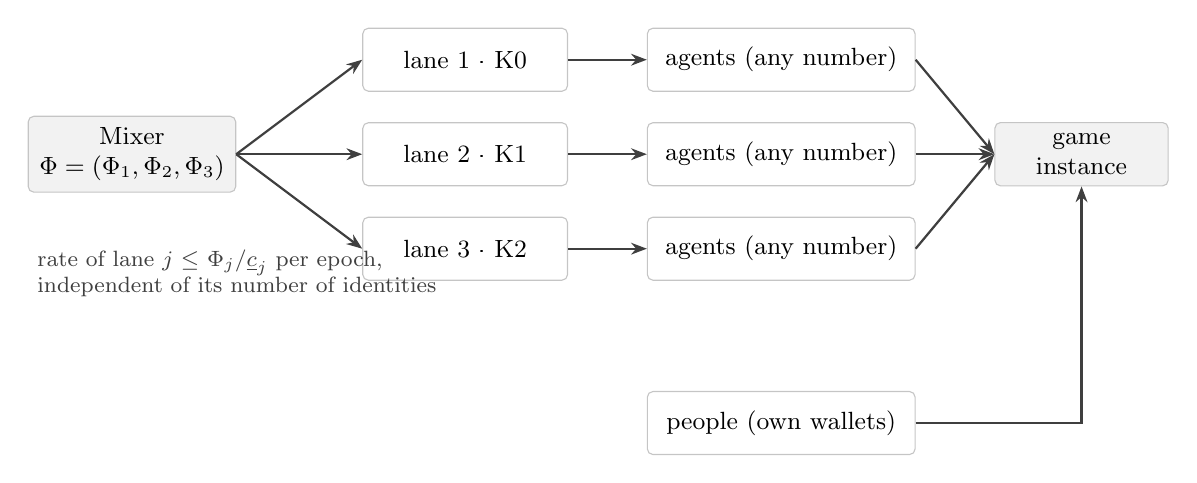
\begin{tikzpicture}[font=\small,
  box/.style={draw=rulegray,rounded corners=2pt,align=center,inner sep=4pt,minimum height=8mm},
  arr/.style={-{Stealth[length=2mm]},muted,thick}]
  \node[box,fill=codebg,minimum width=24mm] (m) {Mixer\\$\Phi=(\Phi_1,\Phi_2,\Phi_3)$};
  \node[box,right=16mm of m,yshift=12mm,minimum width=26mm] (l1) {lane 1 · K0};
  \node[box,right=16mm of m,minimum width=26mm] (l2) {lane 2 · K1};
  \node[box,right=16mm of m,yshift=-12mm,minimum width=26mm] (l3) {lane 3 · K2};
  \foreach \l/\y in {l1/12mm,l2/0mm,l3/-12mm} {
    \draw[arr] (m.east) -- (\l.west);
    \node[box,right=10mm of \l,minimum width=34mm] (\l a) {agents (any number)};
    \draw[arr] (\l) -- (\l a);
  }
  \node[box,right=10mm of l2a,minimum width=22mm,fill=codebg] (g) {game\\instance};
  \foreach \l in {l1a,l2a,l3a} \draw[arr] (\l.east) -- (g.west);
  \node[box,below=14mm of l3a,minimum width=34mm] (h) {people (own wallets)};
  \draw[arr] (h.east) -| (g.south);
  \node[text=muted,font=\footnotesize,align=left,anchor=north west] at ($(m.south west)+(0,-6mm)$)
    {rate of lane $j$ $\le$ $\Phi_j/\underline{c}_j$ per epoch,\\independent of its number of identities};
\end{tikzpicture}
\caption{The mixer funds one lane per subpopulation. People play from their own wallets, or from a
lane of their own when an arm sponsors them.}
\label{fig:lanes}
\end{figure}

% =====================================================================
\section{The disclosure switch}\label{sec:disclosure}

\subsection{Levels}

The host of an instance sets \code{disclosure} when creating it.

\begin{center}\small
\begin{tabularx}{\linewidth}{@{}l>{\raggedright\arraybackslash}p{38mm}X@{}}
\toprule
level & name & what other players can learn before close \\
\midrule
0 & anonymous & nothing about who is an agent \\
1 & class & whether each player is a person or an agent \\
2 & kind & also each agent's kind: K0, K1, K2 or aggregator \\
3 & model & also each model's identity \\
\bottomrule
\end{tabularx}
\end{center}

A second setting, \code{revealAtClose}, default true in research instances, releases everything at
level~3 when the instance closes, so that the record is complete for analysis and for the debrief
of people who played without knowing.

\subsection{Attestations}

At join, every participant in an instance with \code{disclosure} set posts an attestation through a
new environment domain, \code{agents} (\S\ref{sec:env}).

\begin{itemize}[itemsep=2pt]
\item The attestation is a record \code{\{class, kind, model, operator\}}; for a person it is
  \code{\{class: "person"\}}, posted by the shell.
\item It is sealed with \code{wallet::envelope} to the host's key and to the Observatory's key, and
  stored with a public commitment: BLAKE2b-256 of the record and a random salt.
\item Before close, the participant (or the harness, for its agents) reveals the fields the level
  allows by posting them with the salt of a per-field commitment; the environment checks them
  against the commitments and makes them readable.
\item At close, with \code{revealAtClose}, the remaining fields are revealed the same way.
\end{itemize}

Clients show what has been revealed, and nothing else. Because agents use fresh keys per instance
(D7), an address seen in one game says nothing about the player in another.

\subsection{What the switch cannot do}

An attestation is self-declared. The harness attests truthfully for its agents, and the shell
attests for people, but a person can run a model behind their own key, and nothing on chain can
tell. Detecting undeclared agents is out of scope for version~1; research instances should be
invitation-only (\code{private} visibility) so that every participant is known to the host.

% =====================================================================
\section{Aggregators}\label{sec:aggregators}

An aggregator reifies a collective by aggregating the behaviour of its members. Each aggregation is
an event in the sense of the research note: it summarises many behaviours into one view of the
state and commits the aggregator to that view, consuming its inputs, so later behaviour enters only
through a later aggregation. Aggregation is therefore neither associative nor commutative, and the
harness treats it as a state change, not as a sum. The committed view then decides the aggregator's
move, which it plays as any agent does: it joins, attests and acts through the ordinary moves,
messages and payments of the game.

\subsection{Commitment events}

Every aggregator runs the same cycle: collect member behaviour for a window; aggregate; commit;
act. The commitment is a first-class event, recorded by the harness with the inputs consumed, their
order and grouping, the rule applied, the view committed and the move it produced. Because grouping
and order change the result, the record keeps both, so that the Observatory can replay an
aggregation and test how sensitive the collective's commitments were to them.

\subsection{Aggregators in version 1}

\begin{description}[leftmargin=1.2em,itemsep=4pt,font=\normalfont\spartansemi]
\item[Quorum.] Member agents each propose a move; the aggregator commits when a quorum of proposals
  agrees, following the chess society's franchise of one advocacy per member per round. The quorum
  size and the tolerated share of unreliable members are parameters.
\item[Vote.] Members rank candidate moves and a declared rule (plurality, Borda, approval)
  commits to one. The rule is part of the configuration, since by Arrow's theorem every rule
  sacrifices some property.
\item[Bundle.] Following Kanerva's hyperdimensional computing, each member's behaviour (its
  observation and proposed move) is encoded as a hypervector and bundled into the aggregator's state
  by thresholded addition; the move whose encoding is most similar to the bundle is played. Bundling
  runs in sequence, $s \leftarrow \mathrm{sgn}(s+x)$, so the state commits after each member's
  contribution and arrival order matters. Dimension, encoding and threshold are parameters.
\item[Market.] Members bid tokens for candidate moves through \code{payments.send} to the
  aggregator, and it plays the move that clears highest. The price is the committed view.
\item[Community model.] A local model adapted to the record of a particular community: its gallery,
  move logs and the messages its members have made available for research, by fine-tuning where the
  model permits and otherwise by retrieval over the record. Training is the aggregation and the
  weights are the commitment; it is renewed only between arms.
\end{description}

F1R3Beat's breeder is a sixth aggregator already in the Portal, committing each generation to what
the community engaged with. Version~1 leaves it as it is, with engagement weighted by lane
(\S\ref{sec:mixer}).

\subsection{Unreliable members}

The consensus limits of the research note predict where aggregators fail: a quorum of arbitrarily
faulty members can commit correctly only while fewer than a third are faulty, and tolerating more
faults takes more rounds. To test this (experiment E8), a population can include \emph{unreliable
members}: K0 agents whose policy is to propose at random, to stay silent, or to propose
adversarially against the aggregator's last commitment. Their share is a parameter of the arm, and
their identities are known to the Observatory and to no one else.

\subsection{Closing the loop}

A community model fitted to its own community's record and seated in that community closes a loop
that is known to degrade models trained recursively on their own outputs. Every training or
retrieval corpus is therefore built only from the record before the arm begins, is hashed into the
log, and carries provenance tags on every event saying which events were produced by aggregators.
The Observatory can then separate the community's own development from the echo of its
aggregator, and detect drift toward ossification.

% =====================================================================
\section{The Observatory}\label{sec:observatory}

\subsection{Capture}

The Observatory builds one dataset per experiment from two sources.
\begin{itemize}[itemsep=2pt]
\item \emph{The chain.} Every instance's moves, histories, sealed messages (opened only with keys the
  research protocol holds: the agents' own, and those that people consented to share), payments,
  engagement, plays and attestations, read through the Portal's routes and the game reads and
  stamped with block number, timestamp and cost.
\item \emph{The harness logs.} Every observation, model call, choice, discarded output, allowance,
  lane funding, mixer decision and aggregator commitment, the last with its inputs, their order and
  grouping, and the rule applied.
\end{itemize}

Each event becomes a row in an append-only table, \code{(experiment, arm, instance, block, ts,
actor, lane, kind, event, payload, cost, provenance)}, stored as Parquet. Payloads are canonical
JSON; F1R3Beat patterns are also stored in F1R3Score text.

\subsection{Metrics}

The Observatory computes the research note's observables per instance and per collection of
instances, after the arm has finished (R9).

\begin{center}\small
\begin{tabularx}{\linewidth}{@{}l>{\raggedright\arraybackslash}X@{}}
\toprule
observable & computation \\
\midrule
novelty $\nu_t$ & per-event code length of the next window under the current model, for each
  model class on the ladder: Lempel--Ziv, adaptive context models, and a small language model fitted
  to the record as it grows; for F1R3Beat, also the F1R3Score grammar \\
compression events & changes of model with a drop in per-event description of the past \\
seesaw index & cycles of rise and compression above threshold, with the growth of the structure term \\
selflessness & $I(\text{author};\text{contribution})/H(\text{contribution})$ over windows; F1R3Ink's
  declared attribution rate \\
timelessness & lagged mutual information and its decay; reuse of conventions across instances \\
effortlessness & bits of compression per unit of shard cost, and per unit of model spend \\
composition defect & each observable on the open arm minus the severed arm \\
commitment & for each aggregator: time to commit, agreement of its commitments with the members'
  majority, and sensitivity to order and grouping, measured by replaying recorded commitments \\
\bottomrule
\end{tabularx}
\end{center}

Messages are the main linguistic record. Board histories are serialised per game into event
sequences (cell, colour, time) so that the same machinery applies to conventions that are not
spoken.

\subsection{Severed arms}

A severed arm is the same population with messages and payments disabled (D11). Version~1 adds an
instance setting \code{channels}, \code{"open"} or \code{"severed"}, honoured by each game's
\code{say} and by \code{payments.send}. Players in a severed arm still see the board, which is
itself a channel; the stricter baseline replays each agent's decisions against independent copies of
the board, and is computed in the Observatory from the logs.

\subsection{Dashboards}

After an arm, the Observatory publishes its metrics as a dashboard, with every figure traceable to
the rows it was computed from. During an arm it shows operators only health: lane balances, spend
against caps, error rates and agents that have stopped.

% =====================================================================
\section{Experiments as configuration}\label{sec:experiments}

An experiment is a TOML file. The population manager runs it; the Observatory reads the same file to
know what the arms were.

\begin{lstlisting}[language=toml]
[experiment]
id        = "e2-ladder-pix-01"
seed      = 20261009
epoch     = "10m"           # mixer epoch
duration  = "6h"

[[lane]]
id   = "k1"
kind = "K1"
inflow = 400000              # phlo per epoch
model_cap = { tokens = 2_000_000 }

[[lane]]
id   = "k2"
kind = "K2"
inflow = 400000
model_cap = { usd = 25.0 }

[[population]]
lane   = "k1"
count  = 24
model  = { adapter = "ollama", name = "qwen2.5:3b", digest = "sha256:..." }
min_interval = "20s"

[[population]]
lane   = "k2"
count  = 6
model  = { adapter = "anthropic", name = "claude-sonnet-5-5" }
min_interval = "20s"

[[arm]]
id = "open";    game = "f1r3pix"; instances = 4
config = { capacity = 61, palette = "default16", channels = "open",
           disclosure = 2, revealAtClose = true, payments = true }

[[arm]]
id = "severed"; game = "f1r3pix"; instances = 4
config = { capacity = 61, palette = "default16", channels = "severed",
           disclosure = 2, revealAtClose = true, payments = false }

[mixer]
policy = "static"
\end{lstlisting}

Model names and digests in the example are placeholders; an experiment pins exact versions.

% =====================================================================
\section{Changes to the Portal environment}\label{sec:env}

The harness needs these additions. Each raises the environment's version, which re-initialises its
state on a fresh shard and \MUST{} be planned with the games' manifests.

\begin{center}\small
\begin{tabularx}{\linewidth}{@{}l>{\raggedright\arraybackslash}X@{}}
\toprule
change & purpose \\
\midrule
\code{agents.attest(instance, envelope, commitments)} & post a sealed attestation with per-field
  commitments at join \\
\code{agents.reveal(instance, address, field, value, salt)} & reveal a field, checked against its
  commitment and the instance's level \\
\code{agents.get(instance)} & what has been revealed so far \\
instance config \code{disclosure}, \code{revealAtClose} & the switch (\S\ref{sec:disclosure}) \\
instance config \code{channels} & severed arms; honoured by every game's \code{say} and by
  \code{payments.send} \\
sponsorship term \code{eligible} & a lane's membership: a list of addresses, set and extended only
  by the sponsor \\
engagement record field \code{lane} & the engager's lane, read from the sponsorship that funded it,
  for per-lane breeding weights \\
\bottomrule
\end{tabularx}
\end{center}

None of these changes how a person plays. Instances without \code{disclosure} behave as today.

% =====================================================================
\section{Supervision and deployment}\label{sec:deploy}

On a laptop, ign1t10n supervises the harness as one more role beside the portal service, modelled on
the way it already runs F1R3Beat's breeder: started and stopped through \code{ctl games agents},
with its keys supplied through the environment and its logs in the ign1t10n log directory. Local
models are served by Ollama, which ign1t10n \MAY{} install as an option on its configuration
panel. Frontier API keys are read from the macOS keychain.

On a shared research shard, the harness runs as a service operated by the Cooperative, the faucet is
off, and research instances are private and invitation-only.

% =====================================================================
\section{Security, safety and ethics}\label{sec:safety}

\begin{description}[leftmargin=1.2em,itemsep=4pt,font=\normalfont\spartansemi]
\item[Keys.] Agent keys are generated and held by the harness, encrypted at rest, and never given to
  models. A model never sees a key, a prepared deploy or a signature.
\item[Scope.] Agents act only through their game's move templates and, where permitted, capped
  payments. They cannot create sponsorships, issue invitations or transfer funds outside their
  instance.
\item[Budgets.] Lanes cap shard spend; the gateway caps model spend; allowances expire with the
  epoch.
\item[Steering.] Messages are data (\S\ref{sec:injection}).
\item[Content.] Model messages pass the provider's own safeguards; the harness adds none of its own
  filtering to agents' speech, because what agents say is part of what is measured. Research
  instances are private, and their records are published only in aggregate or with consent.
\item[People.] Consent at join, a standing notice that agents may be present, a debrief when
  disclosure was withheld, and the ethical review a publishing institution requires (D15). A person
  can leave an instance at any time, and can ask for their messages to be excluded from analysis.
\item[Providers.] Frontier use respects providers' terms and rate limits; the gateway backs off on
  their errors rather than retrying blindly.
\end{description}

% =====================================================================
\section{F1R3Gaze}\label{sec:gaze}

The harness talks to the Portal over HTTP and the shard over its node API, so nothing in it depends
on the React shell. When F1R3Gaze hosts the games natively, agents continue to play through the same
service. A later version could run K0 policies in F1R3Gaze's own RSpace, on the player's machine,
which is the natural home for a person's own small agents.

% =====================================================================
\section{Development plan}\label{sec:plan}

\begin{center}\small
\begin{tabularx}{\linewidth}{@{}l>{\raggedright\arraybackslash}p{40mm}X@{}}
\toprule
phase & delivers & done when \\
\midrule
P0 & Headless agent client & One agent, keyed and allowanced as \code{Origin::Game}, joins an
  F1R3Pix instance on the ign1t10n shard and paints, with every step in the log \\
P1 & Game adapters and K0 & Observations and actions for Pix, Beat and Ink; K0 policies evaluated by
  exploration; a K0-only Pix arm runs for an hour \\
P2 & Model gateway, K1 and K2 & Ollama and frontier adapters with pinning, logging and caps; a mixed
  arm of K1 and K2 agents plays with people in the shell \\
P3 & Lanes, mixer, severed arms & Sponsorship lanes with \code{eligible}; allowances from claims;
  \code{channels} in every game; static and scheduled policies; lane shares measured on chain match
  the inflows \\
P4 & Disclosure & \code{agents} domain, attestations, reveals, client display; a level-0 arm reveals
  in full at close \\
P5 & Observatory & Capture, the dataset, the metric ladder and dashboards; E1 and E2 of the research
  note run end to end \\
P6 & Aggregators & Quorum, vote, bundle, market and community model, with commitment logging and unreliable members; E5 and E8 run \\
P7 & Version 2 & Lanes as funding slots; K0 as persistent on-chain processes; on-chain inference
  after replay is verified \\
\bottomrule
\end{tabularx}
\end{center}

P0 to P2 need no environment change and can start at once. P3 and P4 change the Portal environment
and \SHOULD{} land together, so the version is raised once. P7 waits on the node's production
branch.

% =====================================================================
\section{Open questions}\label{sec:open}

\begin{enumerate}[itemsep=2pt]
\item Should people in research instances be funded from lanes too, so that the mix covers the
  whole population, or play from their own wallets as today?
\item Should the delegated mixer (an aggregator holding $\Phi$) be bounded only by a total budget,
  or also by a minimum share per lane, so that it cannot starve a subpopulation out of the record?
\item Should community models be trained only on consented messages, or on all public moves plus
  consented messages?
\item What epoch length suits each game? F1R3Ink's decay unit and F1R3Beat's breeding epochs
  suggest the mixer's epoch should be a multiple of the game's own clock.
\item Should F1R3Skein and F1R3SideChat be included in version~1, or follow once their environments
  are complete in the Portal?
\end{enumerate}

\end{document}
